\section{YOLO (You Look Only Once)}
2015 yılında üretilen YOLO (You Look Only Once - Yalnızca bir kez bak) gerçek zaman nesne algılama için kullanılan bir CNN tabanlı bir derin öğrenme algoritmasıdır. YOLO, bir görüntüdeki nesneleri algılamak için kullanılır ve nesnelerin yerlerini ve sınıflarını tahmin eder. YOLO bir görüntüyü tek bir geçişte işleyerek nesneleri algılar, bu da Fast R-CNN, R-CNN gibi diğer nesne algılama yöntemlerine göre daha hızlı çalışmasını sağlar. Algoritma görüntüyü ızgaralara bölerek her bir ızgara içerisinde nesne olup olmadığını ve nesne var ise merkez noktasınının kendi alanı içerisindeki olup olmadığını kontrol eder. Bu işlemden sonra çıktı olarak bir vektör meydana gelir.

\begin{figure}[h]
    \centering
    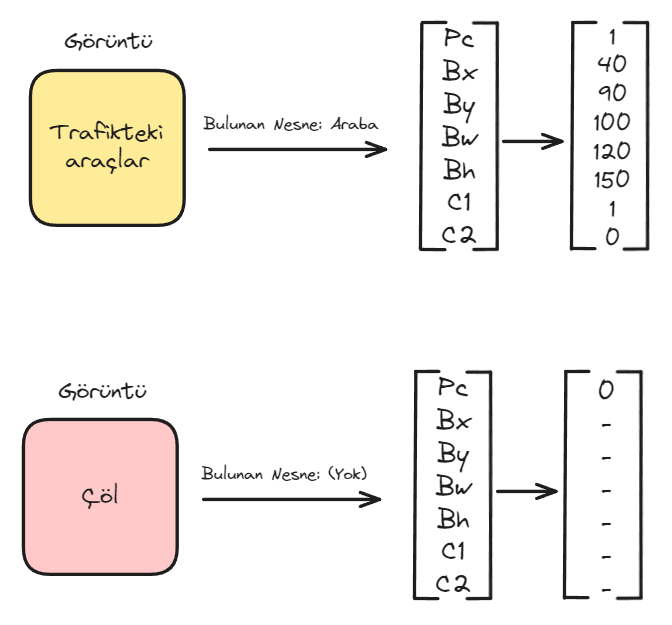
\includegraphics[width=1\textwidth]{images/yolo_vector.png}
    \caption{YOLO nesne algılama vektörü.}
    \label{fig:enter-label}
\end{figure}

Eğer görüntü içerisinde bir nesne varsa aşağıdaki vektör oluşur. Eğer görüntü içerisinde hiçbir nesne yoksa sınıf olasılığı parametresi 0 olur, böylece diğer parametrelerin bir önemi kalmaz.
\begin{itemize}
	\item \textbf{Pc (Probability of Class):} Izgara içerisinde bir nesnenin yer alıp almama olasılığıdır. Nesne var ise 1 yok ise 0'dır.
	\item \textbf{Bx:} Nesnenin merkez noktasının x koordinatıdır.
	\item \textbf{By:} Nesnenin merkez noktasının y koordinatıdır.
	\item \textbf{Bw:} Nesnenin genişliğidir.
	\item \textbf{Bh:} Nesnenin yüksekliğidir.
	\item \textbf{C1:} Tespit  edilen nesnenin sınıfını temsil eder.
	\item \textbf{C2:} Tespit edilen diğer nesnenin sınıfını temsil eder.
\end{itemize}

\subsection{Çalışma Adımları}
\begin{enumerate}
	\item Görüntü küçük parçalara bölünür.
	\item YOLO her bir bölümde potansiyel nesnelerin varlığını ve yerini tahmin eder. Her bölüm için bir dizi çerçeve (bounding box) çizilir. Bu kutular görüntüdeki potansiyel nesnelerin sınırlarını belirtir. Algoritma birden fazla parça içerisinde nesne olduğunu düşünebilir. Bunun sonucunda ortaya ihtiyaç duyulmayan çerçeveler çıkabilir. Bu sorunu önlemek için non-maximum suppression algoritması kullanılır.
	\item YOLO her bir nesne için sınıf belirlemeye çalışır.
	\item Sonuçlar belirli bir güven eşiği altındaki tahminlerin filtrelenmesiyle temizlenir. Bu, düşük güvenilirlikle yapılan tahminleri ortadan kaldırır ve daha doğru sonuçlar elde etmeyi sağlar.
\end{enumerate}

Güven skoru bir nesnenin çerçeve içerisinde ne kadar güvenle bulunduğunu ifade eder. Bu skor, algılanan nesnenin gerçek bir nesne olup olmadığına dair bir ölçüdür. Bir nesnenin güven skoru, o nesnenin tahmin edilen sınıfının doğruluğunu (Pc) ve çerçevenin ne kadar iyi bir şekilde o nesneyi çevrelediğini (IoU - Intersection Over Union) yansıtır. Yüksek güven skoru, nesnenin doğru şekilde algılandığını ve çerçevenin doğru bir şekilde konumlandırıldığını temsil ederken düşük güven skoru, o nesnenin yanlış sınıflandırılığını ve çerçevenin yanlış bir şekilde konumlandırıldığını gösterir.

\[\text{Güven Skoru} = \text{Pr(object)} * \text{IoU}\]

Non-Maximum Suppression (NMS) çoklu çerçevelerin bir nesneyi birden fazla kez algıladığı durumları ifade eder. NMS, birden fazla algılanan nesnelerin yalnızca en güvenilir tahmini olanı tutar. Şu şekilde çalışır;
\begin{enumerate}
	\item Her bir çerçeve güven skoruna göre sıralanır.
	\item En büyük güven skoruna sahip olan çerçeve seçilir ve çıktı listesine eklenir.
	\item Seçilen çerçeve ile diğer çerçeveler arasındaki örtüşme miktarı hesaplanır. Örtüşme miktarı belli bir eşik değerden büyükse yani çerçeveler birbirine çok yakınsa daha düşük güven skoruna sahip olan çerçeveler çıkarılır.
	\item Kalan çerçeveler için bu adımlar tekrarlanır. En yüksek güven skoruna sahip çerçeveler seçilerek çıktı listesine eklenir.
\end{enumerate}

\subsection{YOLO Versiyonları}
\begin{itemize}
	\item \textbf{YOLO V1:} Joseph Redmon ve ekibi tarafından geliştirilmiştir. ImageNet-1000 veri seti ile eğitilmiştir. Darknet mimarisini kullanır. Tek bir CNN modeli kullanır. Küçük nesneleri algılayamaz.
	\item \textbf{YOLO V2 (YOLO9000):} Darknet-19 mimarisini kullanır. Görsel ve derinlik bilgisini işleyen bir multi-scale özellik haritası kullanır. 9000 sınıfın üzerinde nesne tanıyabilir. Görüntüyü 448x448 boyutunda işler.
	\item \textbf{YOLO V3:} Darknet-53 mimarisini kullanır. Atlamalı katmanlar içerir.
	\item \textbf{PP-YOLO:} YOLO V3 modelini temel alır. Darknet-53 mimarisi resnet mimarisi ile değiştirilmiştir ve eğitim grubunda değişiklikler yapılarak bu versiyon elde edilmiştir.
	\item \textbf{YOLO V4:} CSPDarknet53 mimarisini kullanır.  Çıktı süresi küçük bir miktar artırılarak algılama doğruluğu büyük bir derecede artırılmıştır.
	\item \textbf{YOLO V5:} Darknet ağı yerine PyTorch uygulaması olarak geliştirilmiştir. Görüntüyü 640x640 boyutunda işler. 
\end{itemize}

\newpage